% start the document

% specify the document layout and font size
%\documentclass[review,12pt]{elsarticle}
\documentclass[final,12pt]{elsarticle}
\usepackage[margin=1.5cm,includefoot]{geometry}
\usepackage{auto-paper}
\usepackage{enumitem}

% \usepackage{refcheck} %checks for unused labels - comment when done
% %%% Infrastructure    
% \makeatletter
% \newcommand{\refcheckize}[1]{%
%   \expandafter\let\csname @@\string#1\endcsname#1%
%   \expandafter\DeclareRobustCommand\csname relax\string#1\endcsname[1]{%
%     \csname @@\string#1\endcsname{##1}\wrtusdrf{##1}}%
%   \expandafter\let\expandafter#1\csname relax\string#1\endcsname
% }
% \makeatother
% %%%
% %%% Now we add the reference commands we want refcheck to be aware of
% \refcheckize{\cref}
% \refcheckize{\Cref}

% Concatenate the different "values" .tex files
%RMSE values
% \newcommand{\baryrmse}{0.0242}
% \newcommand{\gprrmse}{0.0220}
% \newcommand{\idwrmse}{0.0345}
% \newcommand{\nnrmse}{0.0448}
% \newcommand{\avgrmse}{0.1302}
% %paper-data6
% \newcommand{\baryrmse}{0.0238}
% \newcommand{\gprrmse}{0.0218}
% \newcommand{\idwrmse}{0.0356}
% \newcommand{\nnrmse}{0.0445}
% \newcommand{\avgrmse}{0.1283}
%\newcommand{\gprrmsePercReduction}{83}
% paper-data9
\newcommand{\baryrmse}{0.0239}
\newcommand{\gprrmse}{0.0217}
\newcommand{\idwrmse}{0.0343}
\newcommand{\nnrmse}{0.0448}
\newcommand{\avgrmse}{0.1284}
\newcommand{\gprrmsePercReduction}{83.1}

%MAE values
% \newcommand{\barymae}{0.0145}
% \newcommand{\gprmae}{0.0145}
% \newcommand{\idwmae}{0.0223}
% \newcommand{\nnmae}{0.0307}
% \newcommand{\avgmae}{0.0965}
% %paper-data6
% \newcommand{\barymae}{0.0145}
% \newcommand{\gprmae}{0.0145}
% \newcommand{\idwmae}{0.0225}
% \newcommand{\nnmae}{0.0307}
% \newcommand{\avgmae}{0.0955}
%paper-data9
\newcommand{\barymae}{0.0145}
\newcommand{\gprmae}{0.0145}
\newcommand{\idwmae}{0.0223}
\newcommand{\nnmae}{0.0308}
\newcommand{\avgmae}{0.0959}

%\newcommand{\nnomega}{2.8709 \pm 0.69112}
\newcommand{\nnomega}{2.8702 \pm 0.69117}

\newcommand{\symtime}{76}

\newcommand{\nigprbrkrmse}{0.1471}

%Supplementary
\newcommand{\thr}{\SI{1.1}{\joule\per\square\meter}}
\newcommand{\sigthr}{\SI{1.1}{\joule\per\square\meter}}
\newcommand{\thrtwo}{\SI{1.2}{\joule\per\square\meter}}


%% main-frankenstein-2
\newcommand{\minsymdist}{$\sim$\SI{64.0}{\tobydeg}}
\newcommand{\percExplained}{$\sim$\SI{99.6}{\percent}}
\newcommand{\percFiveVsOne}{$\sim$\SI{70}{\percent}}
\newcommand{\dimOne}{$\sim$\SI{65}{\tobydeg}}

% figure info, etc. that can dynamically change (color of points, etc.)
\newcommand{\startpt}{red points}
\newcommand{\singlept}{magenta points}
\newcommand{\sympt}{dark blue points}
\newcommand{\singlesympt}{dark blue point}
\newcommand{\refpt}{white circle}
\newcommand{\vbordercolor}{black}
\newcommand{\vcellcolor}{light blue}
\newcommand{\inpt}{input}
\newcommand{\outpt}{prediction}
% \newcommand{\inptvar}{ninputpts}
% \newcommand{\distfn}{GBdist4}
\newcommand{\vfzorepo}{\gls{vfz} repository}
\newcommand{\mytitleone}{Five Degree-of-Freedom Property Interpolation of Arbitrary Grain Boundaries via \glsentrytitlecase{vfz}{long} Framework}
% \newcommand{\mytitletwo}{Properties of a \glsentrytitlecase{5dof}{long} \glsentrytitlecase{fz}{long} defined via \glsentrytitlecase{vfz}{long} Framework}
\newcommand{\mytitletwo}{$O_h$ \glsentrytitlecase{5dof}{long} \glsentrytitlecase{fz}{long} Properties via \glsentrytitlecase{vfz}{long} Framework}
\makeglossaries
\GlsXtrEnableEntryCounting{abbreviation}{3}
% \glssetcategoryattribute{abbreviation}{indexonlyfirst}{true}
\glssetcategoryattribute{abbreviation}{nohyper}{true}

% \setabbreviationstyle[abbreviation]{long-short}

% \glsenableentrycount
% \glssetcategoryattribute{abbreviation}{entrycount}{2}

\newabbreviation[longplural=five degrees of freedom]{5dof}{5DOF}{five degree-of-freedom}
\newabbreviation[longplural=three degrees of freedom]{3dof}{3DOF}{three degree-of-freedom}
\newabbreviation[longplural=degrees of freedom]{dof}{DOF}{degree of freedom}
\newabbreviation{ebsd}{EBSD}{electron backscatter diffraction}
\newabbreviation[longplural={grain boundaries}]{gb}{GB}{grain boundary}
\newabbreviation{fcc}{FCC}{face-centered cubic}
\newabbreviation{sem}{SEM}{scanning electron microscope}
\newabbreviation{fea}{FEA}{finite element analysis}
\newabbreviation{bcs}{BCs}{boundary conditions}
\newabbreviation[longplural={triple junctions}]{tj}{TJ}{triple junction}
\newabbreviation{gpr}{GPR}{Gaussian process regression}
\newabbreviation{gprm}{GPRM}{Gaussian process regression mixture}
\newabbreviation{ann}{ANN}{artificial neural network}
\newabbreviation{nn}{NN}{nearest neighbor}
\newabbreviation{rmse}{RMSE}{root mean square error}
\newabbreviation{mae}{MAE}{mean absolute error}
\newabbreviation{brk}{BRK}{Bulatov Reed Kumar}
\newabbreviation{gbed}{GBED}{grain boundary energy distribution}
\newabbreviation{gbcd}{GBCD}{grain boundary character distribution}
\newabbreviation{mfz}{MFZ}{misorientation fundamental zone}
\newabbreviation{bp}{BP}{boundary plane}
\newabbreviation{bpfz}{BPFZ}{boundary plane fundamental zone}
\newabbreviation{knn}{kNN}{k-nearest neighbor}
\newabbreviation{gbe}{GBE}{grain boundary energy}
\newabbreviation{gbo}{GBO}{grain boundary octonion}
\newabbreviation{nbo}{NBO}{no-boundary octonion}
\newabbreviation{oslerp}{oSLERP}{octonion Spherical Linear Interpolation}
\newabbreviation{loocv}{LOOCV}{leave-one-out cross validation}
\newabbreviation{kfcv}{kFCV}{k-fold cross validation}
\newabbreviation{seo}{SEO}{symmetrically equivalent octonion}
\newabbreviation{fex}{FEX}{file exchange}
\newabbreviation{idw}{IDW}{inverse-distance weighting}
\newabbreviation{fic}{FIC}{fully independent conditional}
\newabbreviation{svd}{SVD}{singular value decomposition}
\newabbreviation{gbc}{GBC}{grain boundary character}
\newabbreviation{fz}{FZ}{fundamental zone}
% \newabbreviation{pfz}{pFZ}{pseudo fundamental zone} % pfz replaced by vfz
% \newabbreviation{cmo}{CMO}{closed-mesh octonion} % cmo replaced by vfzo
\newabbreviation{vfz}{VFZ}{Voronoi fundamental zone}
\newabbreviation{vfzgbo}{VFZ-GBO}{Voronoi fundamental zone grain boundary octonion}
\newabbreviation{lobpcg}{LOBPCG}{locally optimal block preconditioned conjugate gradient}
\newabbreviation{lkr}{LKR}{Laplacian kernel regression}
\newabbreviation{ms}{MS}{molecular statics}
\newabbreviation{sst}{SST}{standard stereographic triangle}
\newabbreviation{ml}{ML}{machine learning}
\newabbreviation{doe}{DoE}{design of experiments}
\newabbreviation{ct}{CT}{coherent-twin}
% example abbreviations
% \newabbreviation{seo}{SEO}{symmetrically equivalent octonions}
%\newabbreviation[longplural={grain boundaries}]{gb}{GB}{grain boundary}

%example usage: \gls{gpr}
%example usage: \Gls{gpr} (capitalize first letter, only meaningful for first usage)
% \glspl{seo} --> symmetrically equivalent octonions OR SEOs
%^^^^^^^^^^^^^^^^^^^^^^^^^^^^^^^^^^^^^^^^^^^^^^^^^^^


\begin{document}
	
	\sloppy %to hopefully deal with whitespace better
	
	\begin{frontmatter}
		
		%\title{Grain Boundary Octonion Meshing and Interpolation}
		\title{N-Sphere Barycentric Interpolation: A 7-Sphere with 2D Visualizations}
		
		\author[myu]{Sterling G. Baird\corref{cor1}}
\ead{ster.g.baird@gmail.com}
\author[myu]{Eric R. Homer}
\author[myu]{David T. Fullwood}
\author[myu]{Oliver K. Johnson}

\address[myu]{Department of Mechanical Engineering, Brigham Young University, Provo, UT 84602, USA}

\cortext[cor1]{Corresponding author.}

\date{October 2021}
		
		\begin{abstract}
			We present a method for performing efficient barycentric interpolation for large point sets which reside on the surface of a hypersphere. This method includes removal of degenerate dimensions via \gls{svd} transformations and linear projections, determination of intersecting facets via \gls{nn} searches, and interpolation. This method is useful for hyperspherical point sets for applications such as \glspl{gb} structure-property models, robotics, and specialized neural networks. Corresponding MATLAB code is available at \url{github.com/sgbaird-5dof/interp}.
		\end{abstract}
	
	\begin{keyword}
		barycentric \sep interpolation \sep hypersphere \sep octonion \sep triangulation % \sep Metastability \sep Grain Boundary Distance \sep Grain Boundary Energy
	\end{keyword}

	\end{frontmatter}

\section{Introduction}
Barycentric coordinates are a type of homogeneous coordinate system that reference a \outpt{} point within a simplex \cite{langerSphericalBarycentricCoordinates2006} or convex polytope \cite{floaterGeneralizedBarycentricCoordinates2015,meyerGeneralizedBarycentricCoordinates2002,langerSphericalBarycentricCoordinates2006} based on "masses" or weights at the vertices, which can be negative. The \outpt{} point is assumed to be the barycenter (center of mass) of the simplex or convex polytope, and weights at the vertices necessary to make this assumption true are determined. We utilize rigid \gls{svd} transformations and a standard triangulation algorithm\footnote{i.e. quickhull \cite{barberQuickhullAlgorithmConvex1996} via \matlab{delaunayn()} in \matlab{sphconvhulln.m}. Built-in MATLAB functions are indicated with parantheses (e.g. \matlab{delaunayn()}), whereas custom functions are indicated with the \matlab{.m} extension (e.g. \matlab{sphconvhulln.m}). } to define a simplicial mesh on the surface of an n-dimensional hypersphere (\cref{sec:app:bary:tri}). We then use barycentric weights (i.e. coordinates) for computing intersections of a point within a simplicial facet (\cref{sec:app:bary:int}) and for interpolation (\cref{sec:app:bary-interp}) \cite{langerSphericalBarycentricCoordinates2006}. These methods are relevant for applications such as \glspl{gb} structure-property models \cite{chesserLearningGrainBoundary2020}, robotics hand-eye calibration \cite{wuHandEyeCalibration4D2020}, and efficient neural networks \cite{wuDeepOctonionNetworks2020}, especially cases where coordinates may have degenerate dimensions, occupy no more than a hemisphere\footnote{When the points occupy less less than a hemisphere, a linear projection onto a hyperplane followed by an \gls{svd} transformation can be used to compute the triangulation in one dimension lower. If the points span the full hypersphere, triangulation must proceed in the original dimensionality to produce an accurate triangulation. }, or require interpolation of properties. While the methods described are general to n-dimensional hyperspheres, we focus on one application of interest: the unit 7-sphere. For further information on barycentric coordinates and its applications and generalizations, see \cite{anisimovSubdividingBarycentricCoordinates2016,budninskiyPowerCoordinatesGeometric2016,dyerBarycentricCoordinateNeighbourhoods2016,floaterGeneralizedBarycentricCoordinates2015,floaterInjectivityWachspressMean2010,hormannDiscretizingWachspressKernels2017,hormannMaximumEntropyCoordinates2008,langerHigherOrderBarycentric2008,langerSphericalBarycentricCoordinates2006,leiNewCoordinateSystem2020,meyerGeneralizedBarycentricCoordinates2002,peixotoVectorFieldReconstructions2014,pihajokiBarycentricInterpolationRiemannian2019,rustamovBarycentricCoordinatesSurfaces2010,skalaRobustBarycentricCoordinates2013,taoFastNumericalSolver2019,warrenBarycentricCoordinatesConvex2007}.
%
% Our barycentric interpolation approach includes:
% \begin{itemize}%[nolistsep]
% 	\item[1.] triangulation of a mesh (\cref{sec:app:bary:tri})
% 	\item[2.] finding intersections (\cref{sec:app:bary:int})
% 	\item[3.] calculating interpolated values (\cref{sec:app:bary-interp})
% \end{itemize}
%
\section{Triangulating a Mesh}
\label{sec:app:bary:tri}

Creation of a simplicial mesh is necessary to perform barycentric interpolation. Due to the difficulty of visualizing a high-dimensional n-sphere, we provide visual illustrations of the process as applied to lower-dimensional analogues. The triangulation process occurs by:
\begin{enumerate}%[nolistsep]
	\item[1.1] applying a \gls{svd} transformation to remove any degeneracies\footnote{e.g. U(1)-symmetry degeneracy for \glspl{gbo} \cite{francisGeodesicOctonionMetric2019}) inherent in the coordinates} (\cref{sec:app:bary:tri:svd1}
	\item[1.2] linearly projecting points onto a hyperplane that is tangent to the vector between the origin and the mean of the \inpt{} points\footnote{This applies when the data resides on less than a hemisphere and is to reduce computational burden of the triangulation. } (\cref{sec:app:bary:tri:project})
	\item[1.3] performing a second \gls{svd} transformation (\cref{sec:app:bary:tri:svd2})
	\item[1.4] computing the triangulation according to the quickhull algorithm \cite{barberQuickhullAlgorithmConvex1996}
\end{enumerate}

In the explanation of each step that follows, we make reference to lower-dimensional visual analogues of the triangulation procedure, which are given in \cref{fig:bary-remove-deg,fig:bary-delaunay,fig:bary-interp}. We note that 3D Cartesian coordinates in \cref{fig:bary-remove-deg} correspond to 8D Cartesian coordinates, whereas 3D Cartesian coordinates in \cref{fig:bary-delaunay,fig:bary-interp} correspond to 7D Cartesian coordinates. This is intentional for two reasons.

First, \cref{fig:bary-remove-deg} illustrates that 8D Cartesian points constrained to the surface of a hypersphere are analogous to a point cloud on the 2-sphere (\cref{fig:bary-remove-deg}a) and that an 8D Cartesian point set constrained to the surface of a hypersphere is analogous to a geodesic arc on the 2-sphere (\cref{fig:bary-remove-deg}b). If a point set has a degenerate dimension, this can be removed by a rigid \gls{svd} transformation to 7D Cartesian coordinates (analogous to 2D Cartesian coordinates in \cref{fig:bary-remove-deg}c). This sequence would be more difficult to visualize if \cref{fig:bary-remove-deg}a was meant to represent a point cloud on the 3-sphere (4D Cartesian coordinates), etc.

Second, \cref{fig:bary-delaunay} illustrates a second transformation from normalized 7D Cartesian coordinates (\cref{fig:bary-delaunay}a) to a hyperplane (\cref{fig:bary-delaunay}b) which is then transformed into 6D Cartesian coordinates via a second \gls{svd}. In this case, key issues are retained that would otherwise be lost if an arc on a circle (1-sphere) to 1D Cartesian coordinates were used instead\footnote{Non-intersection issues due to high-aspect ratios and consideration of facets connected up to \matlab{nnMax} \glspl{nn} do not manifest in triangulations on the surface of a 1-sphere because one of the two facets (i.e. line segments) connected to the first \gls{nn} mesh vertex relative to the \outpt{} point is guaranteed to have an intersection.}. Additionally, the use of actual triangles is a more familiar and compelling illustration of \textit{triangulation}.

\begin{figure*}
	\centering
	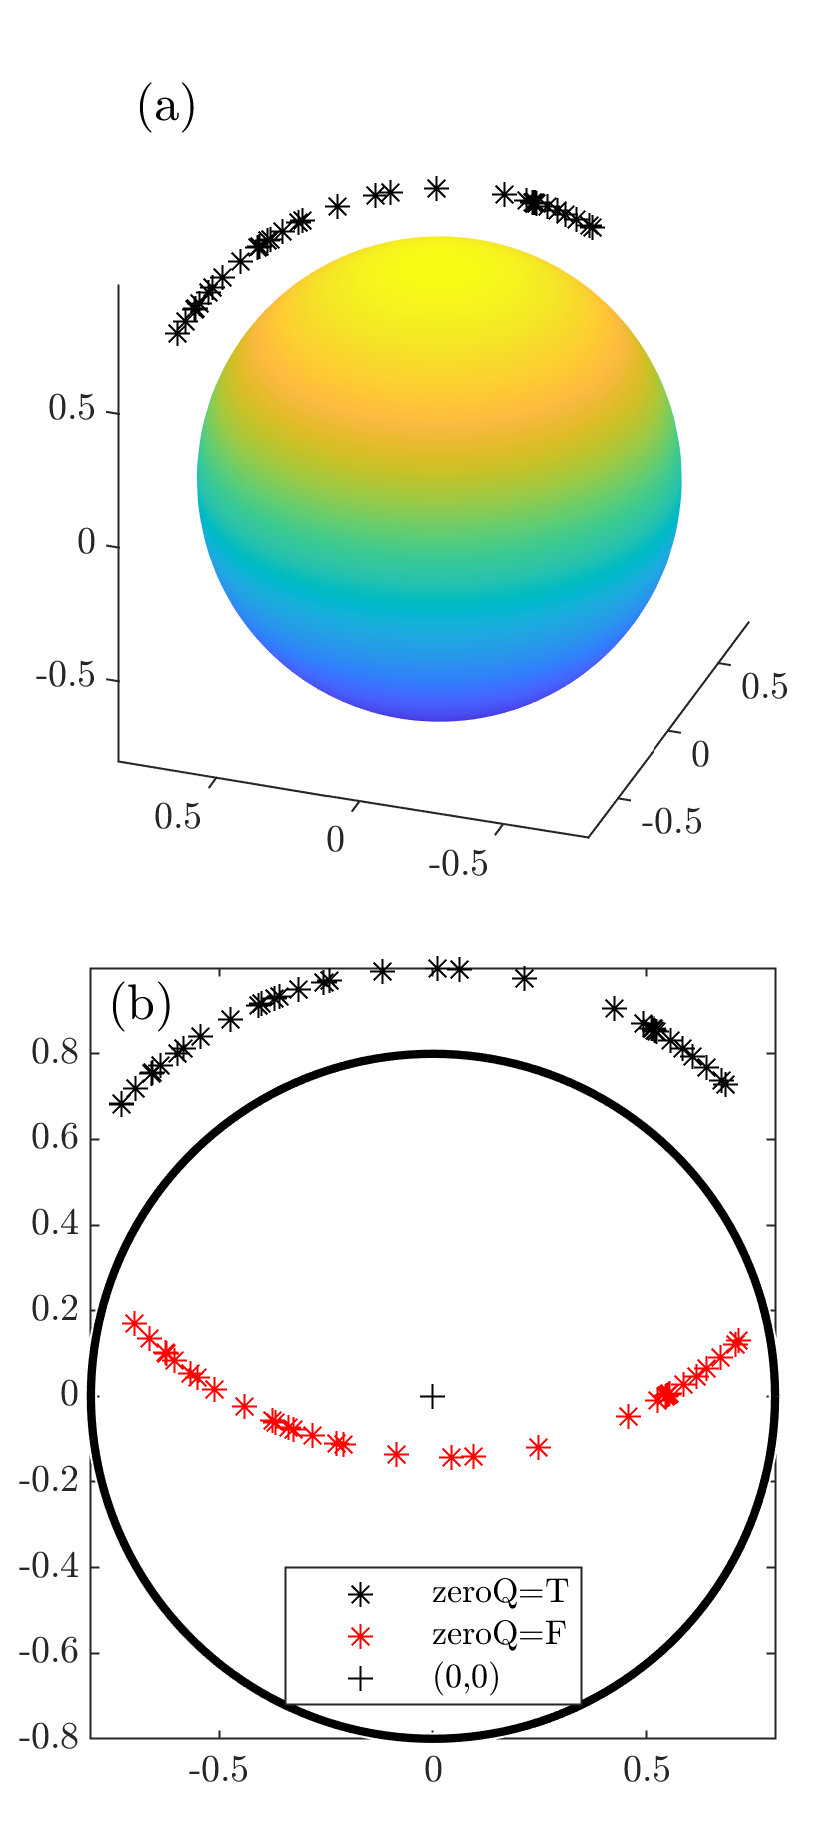
\includegraphics[scale=0.9]{bary-remove-deg.png}
	\caption{3D Cartesian to 2D Cartesian analogue of 8D Cartesian to 7D Cartesian degeneracy removal via rigid \gls{svd} transformation as used in barycentric interpolation approach. (a) Starting spherical arc points on surface of 2-sphere, (b) rotational symmetrization applied w.r.t. z-axis (analogous to U(1) symmetrization), and (c) degenerate dimension removed via \glsxtrlong{svd} transformation to 2D Cartesian with either the origin (black plus) preserved (black asterisks, \matlab{zeroQ=T}) for triangulation or ignored (red asterisks, \matlab{zeroQ=F}) for mesh intersection. The spheres (a,b) and circle (c) each have a radius of 0.8 and are used as a visualization aid only.}
	\label{fig:bary-remove-deg}
\end{figure*}

\begin{figure*}
	\centering
	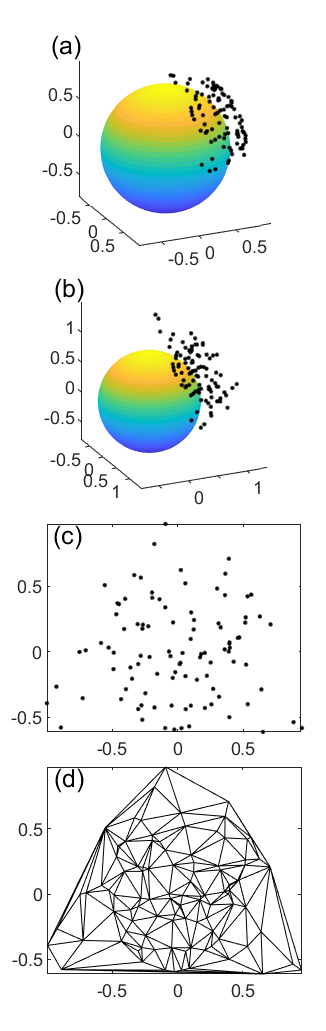
\includegraphics[scale=1]{bary-delaunay.png}
	\caption{3D Cartesian to 2D Cartesian analogue of 7D Cartesian to 6D Cartesian mesh triangulation used in barycentric interpolation approach. (a) 3D Cartesian \inpt{} points are (b) linearly projected onto hyperplane that is tangent to mean of starting points. (c) The degenerate dimension is removed via a rigid \gls{svd} transformation to 2D Cartesian and the Delaunay triangulation (black lines) is calculated, with \inpt{} vertices (red). Delaunay triangulation superimposed onto normalized \inpt{} points (d). The spheres in (a), (b), and (d) have a radius of 0.8 and are used for visualization only.}
	\label{fig:bary-delaunay}
\end{figure*}

While lower dimensional analogues are useful for visualizing and understanding the process of triangulation, a written description for the full-dimensional space is also given (\cref{sec:app:bary:tri:svd1,sec:app:bary:tri:project,sec:app:bary:tri:svd2}). As appropriate, we refer back to the teaching figures described in this section.

\subsection{\glsentrytitlecase{svd}{long} Transformation from 8D Cartesian to 7D Cartesian}
\label{sec:app:bary:tri:svd1}
To reduce the computational complexity of triangulating a high-dimensional mesh \cite{barberQuickhullAlgorithmConvex1996}, some simplifications are made. First, the degenerate dimension (e.g. obtained from analytically minimizing $U(1)$ symmetry \cite{francisGeodesicOctonionMetric2019}) is removed via a rigid (i.e. distance- and angle-preserving) \gls{svd} transformation,
%to enable use of MATLAB's quickhull \cite{barberQuickhullAlgorithmConvex1996} implementations such as \matlab{delaunayn} and \matlab{convhulln}. Removal of the degenerate dimension is done via a rigid \gls{svd} transformation,
analogous to a Cartesian rotation and translation (see 3D to 2D \gls{svd} transformation from \cref{fig:bary-remove-deg}b to \cref{fig:bary-remove-deg}c).
%Thus, a set of \glspl{gbo} originally represented by 8D Cartesian coordinates are collapsed to a 7D Cartesian representation while preserving both distances and angles among the points
A \gls{svd} is given by:
\begin{equation} \label{eq:svd-cond}
	A=\text{USV}'
\end{equation}
where $U$, $S$, $V$, and $\cdot '$ represent a unitary matrix with sorted, singular vectors, a diagonal matrix containing sorted, singular values, a unitary matrix with sorted, singular vectors, and Hermitian transpose operator, respectively.
The \gls{svd} transformed coordinates \cite{anatoliyCheckIfRay2015} are given by:
\begin{equation} \label{eq:svd-force}
	\overbrace{\left(
\begin{array}{cccc}
 b_{1,1} & b_{1,2} & \ldots  & b_{1,n-n_\text{deg}} \\
 b_{2,1} & b_{2,2} & \ldots  & b_{2,n-n_\text{deg}} \\
 \vdots  & \vdots  & \ddots & \vdots  \\
 b_{m,1} & b_{m,2} & \ldots  & b_{m,n-n_\text{deg}} \\
\end{array}
\right)}^B=\overbrace{\left(
\begin{array}{cccc}
 u_{1,1} & u_{1,2} & \ldots  & u_{1,n} \\
 u_{2,1} & u_{2,2} & \ldots  & u_{2,n} \\
 \vdots  & \vdots  & \ddots & \vdots  \\
 u_{m,1} & u_{m,2} & \ldots  & u_{m,n} \\
\end{array}
\right)}^U \overbrace{\left(
\begin{array}{cccc}
 s_{1,1} & s_{1,2} & \ldots  & s_{1,n-n_\text{deg}} \\
 s_{2,1} & s_{2,2} & \ldots  & s_{2,n-n_\text{deg}} \\
 \vdots  & \vdots  & \ddots & \vdots  \\
 s_{n,1} & s_{n,2} & \ldots  & s_{n,n-n_\text{deg}} \\
\end{array}
\right)}^{S_{\text{sub}}}
\end{equation}
where $n_\text{deg}$ and $S_{\text{sub}}$ represent number of degenerate dimensions and $S$ with the degenerate columns removed, respectively.
%
\subsection{Linearly Project onto Hyperplane}
\label{sec:app:bary:tri:project}
Next, the resulting 7D Cartesian representation of each point is projected onto a hyperplane that is tangent to the centroid (i.e. mean) of the point set\footnote{This is \textit{not} a rigid transformation; however, it approximates one with sufficient accuracy to produce a high-quality triangulation.} (\cref{fig:bary-delaunay}a). The linear projection is given by \cite{anatoliyCheckIfRay2015}:
\begin{equation} \label{eq:linear-proj}
	a=-\frac{p \| v\| }{v.p}
\end{equation}
where $\text{v}$ and $\text{unit normal to hyperplane of interest}$ represent p and point to project from hypersphere to hyperplane, respectively.
By performing this linear projection, one of the dimensions becomes degenerate.

\subsection{\glsentrytitlecase{svd}{long} Transformation from 7D Cartesian to 6D Cartesian}
\label{sec:app:bary:tri:svd2}
This additional degeneracy is removed via a second \gls{svd} transformation, this time to 6D Cartesian coordinates (see 3D to 2D projection in \cref{fig:bary-delaunay}a-b). Finally, the resulting points can be triangulated via the quickhull algorithm \cite{barberQuickhullAlgorithmConvex1996}\footnote{See \matlab{sphconvhulln.m} and \matlab{delaunayn()}}, which relies on Euclidean distances\footnote{While the triangulation algorithm used in this work relies on Euclidean distances, other distance metrics that are non-Euclidean \cite{morawiecDistancesGrainInterfaces2019} could potentially be incorporated into the barycentric approach such as by doing an edge-length based simplex reconstruction \cite{connorHighdimensionalSimplexesSupermetric2017,boissonnatOnlyDistancesAre2017} using the triangulation edge lengths.}. Because the simplicial mesh is defined by a list of edges between vertices for each simplicial facet, this list applies immediately to the point set in its 7D Cartesian coordinates (i.e. no reverse transformation is necessary to use the mesh on the 6-sphere in 7D).

\section{Intersections in a Mesh}
\label{sec:app:bary:int}

Once the triangulation has been determined, we need to find which facet each \outpt{} point intersects (i.e. find the intersecting facet). There are two sub-steps:
\begin{itemize}%[nolistsep]
	\item[2.1] apply the same rigid transformation to the \outpt{} points as was applied to the \inpt{} points (otherwise the \outpt{} points won't line up properly with the mesh) (\cref{sec:app:bary:int:out-svd})
	\item[2.2] identify facets nearby a \outpt{} point and test for intersection (\cref{sec:app:bary:int:facets}).
\end{itemize}
\subsection{Apply Same \glsentrytitlecase{svd}{long} to Input and Prediction Points}
\label{sec:app:bary:int:out-svd}
The positions of the \outpt{} points need to be fixed relative to the mesh even after the rigid \gls{svd} transformation. %Thus, it is crucial to perform the same rigid \gls{svd} transformation (i.e. same rotation and translation) on the \outpt{} points as was applied to the \inpt{} points.
This is accomplished by:
\begin{itemize}%[nolistsep]
	\item[2.1a] concatenating both \inpt{} and
	\outpt{} points
	\item[2.1b] performing the \gls{svd} transformation\footnote{See  \matlab{proj\_down.m} via \matlab{svd()}}
	\item[2.1c] subsequently separating the transformed \inpt{} and \outpt{} points (reverse of concatenation step)
\end{itemize}
%
The same \gls{svd} transformation can be applied without major issue to new points, assuming the new points are not positioned outside the bounds of the original convex hull\footnote{To map new points onto the mesh, the \matlab{usv} structure output from \matlab{proj\_down.m} needs to be stored and supplied in future calls to \matlab{proj\_down.m}. Likewise, \matlab{usv} need to be supplied to \matlab{proj\_up.m} to perform the reverse \gls{svd} transformation.}.
%
\subsection{Testing Nearby Facets for Intersections}
\label{sec:app:bary:int:facets}
Once the \outpt{} points are lined up properly with the mesh, the facet containing the \outpt{} point (i.e. intersecting facet) is found\footnote{Testing intersections for nearby facets is handled in \matlab{intersect\_facet.m} and depends on the barycentric coordinate computations in \matlab{projray2hypersphere.m}.}. We define the intersecting facet as the one for which a point's barycentric coordinates are positive within a given tolerance:
\begin{equation} \label{eq:projtol}
	\lambda _i\text{$\geq $-$\sigma $,i$\in $[1,d]}
\end{equation}
where $\text{$\$\backslash \backslash $lambda$\$$}$ and $\text{i-th barycentric coordinate}$ represent $\sigma$ and projection (or intersection) tolerance, respectively.Consequently, we determine facet affiliation by:
\begin{enumerate}%[nolistsep]
	\item[2.2a] linearly projecting the \outpt{} point onto the hyperplane defined by a mesh facet's vertices (\cref{fig:bary-interp})
	\item[2.2b] computing\footnote{See \matlab{projray2hypersphere.m}} the point's barycentric coordinates within the facet \cite{anatoliyCheckIfRay2015,skalaRobustBarycentricCoordinates2013}
	\item[2.2c] testing that all coordinates are positive \cite{langerSphericalBarycentricCoordinates2006} within a tolerance\footnote{Two tolerances\footnote{We typically use \matlab{projtol=1e-4} in \matlab{proj_down.m} and \matlab{inttol=1e-2} in \matlab{intersect_facet.m}, respectively. } are used: one for the initial computation of barycentric coordinates by projecting onto the hypersphere to determine facet affiliation and a larger tolerance for computation of barycentric coordinates to determine interpolated values (\cref{sec:app:bary-interp}). }
	\item[2.2d] repeating steps 2.2a-2.2c until an intersection is found or a stop condition is reached\footnote{The stop condition is that up to a certain number of \gls{nn} have been considered (or all points have been considered). The parameter associated with this is \matlab{nnMax} in \matlab{intersect_facet.m} }
\end{enumerate}

\begin{figure}
	\centering
	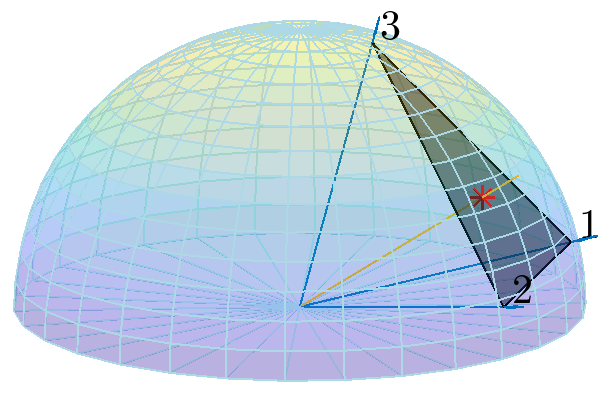
\includegraphics[scale=1]{bary-interp.png}
	\caption{A ray (red line) is linearly projected from the 2-sphere onto the hyperplane of a mesh facet (transparent black), shown as a red asterisk. The barycentric coordinates are computed as $\lambda_{i \in [1,3]} = \frac{1}{3}$. Because all barycentric coordinates are positive, it is determined that the projected point is an intersection with the mesh. Given vertex values of \num{8.183}, \num{3.446}, and \num{3.188} for vertices 1, 2, and 3, respectively, the interpolated value is calculated as \num{4.94} via \cref{eq:bary-interp}.}
	\label{fig:bary-interp}
\end{figure}
%
%For further information on barycentric coordinates and its applications and generalizations, see \cite{anisimovSubdividingBarycentricCoordinates2016,budninskiyPowerCoordinatesGeometric2016,dyerBarycentricCoordinateNeighbourhoods2016,floaterGeneralizedBarycentricCoordinates2015,floaterInjectivityWachspressMean2010,hormannDiscretizingWachspressKernels2017,hormannMaximumEntropyCoordinates2008,langerHigherOrderBarycentric2008,langerSphericalBarycentricCoordinates2006,leiNewCoordinateSystem2020,meyerGeneralizedBarycentricCoordinates2002,peixotoVectorFieldReconstructions2014,pihajokiBarycentricInterpolationRiemannian2019,rustamovBarycentricCoordinatesSurfaces2010,skalaRobustBarycentricCoordinates2013,taoFastNumericalSolver2019,warrenBarycentricCoordinatesConvex2007}.
%
Due to the large number of facets per point of a high-dimensional triangulation (approximately \num{2000} facets per vertex for a \num{50000} point triangulation, or \num{1e8} total facets), some simplifications are made in order to determine intersections of \outpt{} points with the mesh. If every edge length of every facet were equal, only facets connected to the first \gls{nn} would need to be considered to find a proper intersection. However, since the points are randomly sampled, edge lengths of facets are non-uniform, and non-unity aspect-ratio facets exist (\cref{fig:bary-delaunay}, \cref{fig:high-aspect-non-int}). If the facets have high-aspect ratios, the intersecting facets of \outpt{} points can be far from the \glspl{nn} mesh points relative to the \outpt{} points (see \cref{fig:high-aspect-non-int} inset), especially near the perimeter of a hyperspherical surface mesh. Rather than loop through every facet to find an intersection ($\sim$\num{1e8} facets in a \num{50000} point mesh), the \outpt{} point intersections are calculated by considering facets connected to up to some number of \gls{nn} mesh vertices\footnote{See \matlab{nnMax} in \matlab{intersect_facet.m}. We have typically used \matlab{nnMax=10}. } relative to each \outpt{} point. The \gls{nn} mesh vertices relative to a \outpt{} point are computed. The facet IDs of facets connected to these \glspl{nn} are then computed\footnote{via \matlab{find(K==nn)}, where \matlab{K} is the triangulation from \matlab{sphconvhulln.m} and \matlab{nn} is the ID of one of the \gls{nn} mesh vertices)}.

Some \outpt{} points will have no intersecting facet found.
%(which can occur just outside the piece-wise linear perimeter of the mesh due to finite resolution)
From our numerical testing, we determine that this non-intersection phenomenon occurs in two situations:
\begin{itemize}%[nolistsep]
	\item high-aspect ratio facets (described above)
	\item \outpt{} points that are positioned just outside the bounds of the mesh but within the bounds of a region, due to the fact that the mesh is a piecewise linear approximation of a surface with a curved perimeter and that randomly sampled points typically do not fall on the true perimeter
\end{itemize}
In the first case, barycentric interpolation within high-aspect ratio facets may actually lead to worse interpolation error than a \gls{nn} interpolation strategy due to influence by points far from the \outpt{} point. In the second case, there is no true intersection between the \outpt{} point and the mesh. Both issues can be addressed with the same strategy: we apply a \gls{nn} approach when an intersecting facet is not found within some number of \glspl{nn}. In numerical tests, meshes composed of \num{388} and \num{50000} vertices produced non-intersection rates of \SI{12.07 \pm 1.02}{\percent} and \SI{0.68 \pm 0.11}{\percent}, respectively, over approximately \num{10} trials and using \num{10000} \outpt{} points for each trial. An alternative strategy for the second case is to linearly project the point of interest onto the closest facet, and compute the interpolation there.
%
% \subsection{High-Aspect Ratios}
% \label{sec:supp:bary:artifact}
% An artifact of the barycentric interpolation method which occurs due to the presence of high-aspect ratio facets is shown in \cref{fig:high-aspect-non-int}. As the dimensionality increases for a constant number of points and from our numerical tests, the rate of missed facet intersections increases. This artifact and our method for addressing it are discussed in \cref{sec:app:bary:int}.
%
\section{Interpolation}
\label{sec:app:bary-interp}

Once a mesh triangulation has been determined (\cref{sec:app:bary:tri}), barycentric coordinates are recomputed for a \outpt{} point within the \inpt{} mesh (\cref{sec:app:bary:int}) using a somewhat larger tolerance; the interpolated value is found by taking the dot product of the \outpt{} point's barycentric coordinates and the properties of the corresponding vertices of the intersecting facet via
\begin{equation}
	\label{eq:bary-interp}
	v_{m,q}=\underset{i=1}{\overset{N}{\sum }}\lambda _{m,i} v_{m,i}
\end{equation}
where $\lambda_{m,i}$, $v_{m,q}$, $v_{m,i}$ and $N$, are the barycentric coordinates of the m-th \outpt{} point, interpolated property at the m-th \outpt{} point, property of the $i$-th vertex of the intersecting facet for the m-th \outpt{} point, and number of vertices in a given facet ($N = 7$ for facets of the simplicial mesh on the degeneracy-free 6-sphere), respectively. Interpolation of many \outpt{} points simultaneously can be accomplished by a simple, vectorized approach\footnote{i.e. \matlab{dot()} as used in \matlab{interp\_bary\_fast.m}}. This assumes triangulation and weights have been precomputed. In other words, both \inpt{} and \outpt{} coordinates remain fixed, and only \inpt{} property values change. If this is the case, barycentric interpolation of new points is incredibly fast. By contrast, if \inpt{} coordinates change, the triangulation must be recomputed, and if \outpt{} coordinates change, the intersecting facets must be recomputed. Both triangulation and finding intersecting facets are computationally demanding with respect to memory and runtime for large datasets. For example, a mesh triangulation consisting of \num{50000} points evaluated for \num{10000} interpolation points requires $\sim$1.6~hours using 12 cores ($\sim$20~CPU~hours in total) with \num{128}~GB of RAM available. The total runtime as a function of set size evaluated on \num{10000} \outpt{} points (i.e. combined triangulation and intersection finding) is estimated by a fitted linear model\footnote{Using Mathematica's \texttt{FindFormula[]} }, $5332.02 + 1.26959 x$, where $x$ is the number of points and $1000\leq x \leq 50000$. The triangulation itself ($\sim$\num{1e8} facets) requires $\sim$6~GB of memory storage.

\begin{figure*}
	\centering
	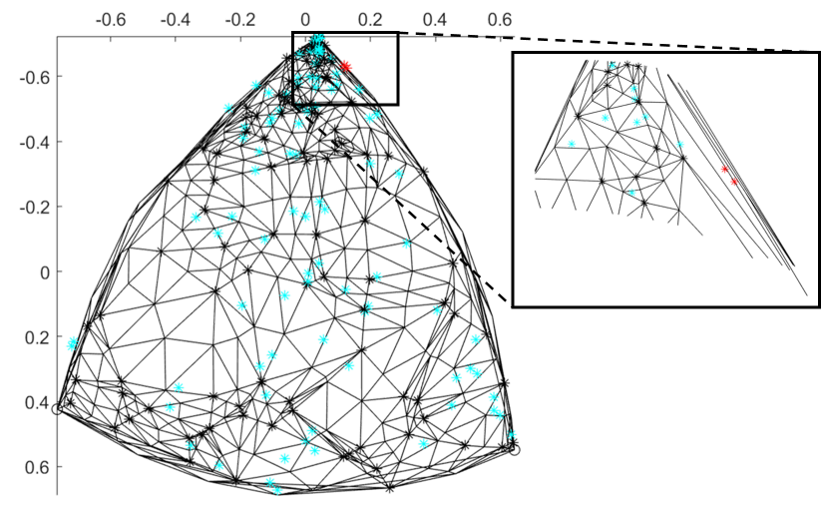
\includegraphics[scale=0.8]{figures/high-aspect-non-int.png}
	\caption{Illustration of two \outpt{} points (red) for which no intersecting facet is found due to being positioned within a high-aspect ratio facet. The inset shows that facets connected to the \gls{nn} do not contain the \outpt{} point. Many \glspl{nn} would need to be considered before an intersection is found. Additionally, it is expected that if found, the interpolation will suffer from higher error due to use of facet vertices far from the interpolation point. Proper intersections of \outpt{} points with the mesh are shown in blue.}
	\label{fig:high-aspect-non-int}
\end{figure*}
%
% \section{Conclusion}
% \Gls{svd} transformations, linear projections, and \gls{nn} searches can be used to reduce the computational burden of high-dimensional hyperspherical triangulations and intersection-finding. Large point sets in high-dimensions still have large memory and runtime requirements, but are more tractable with these methods. When the borders of the region of interest are not within the convex hull of points or when the region of interest is inherently curved (beyond the curvature naturally present due to residing on a hypersphere), non-intersections manifest and can be addressed by defaulting to a \gls{nn} approach.
%
\section*{Acknowledgements}
We thank Victoria Baird for useful discussions related to the visualization and triangulation of hyperspherical meshes. This work was supported by the National Science Foundation under Grant No. 1610077. This work was supported in part through computational resources provided by Brigham Young University's Office of Research Computing.
% \printglossaries
%
\bibliographystyle{elsarticle-num-names}
\begingroup
    \setlength{\bibsep}{10pt}
    \setstretch{1}
    \bibliography{5dof-gb-energy.bib}
\endgroup

\end{document}